\chapter{Apresentação do Modelo}
\label{modelo}

Conforme explicado na Seção \ref{fundamentacao:redes:construcao}, a construção de uma \textit{Rede Bayesiana} pode ser dividada em duas fases: a construção do GAD, e a definição das funções de probabilidade. Portanto, neste capítulo, serão descritas essas duas fases do processo de construção do modelo proposto neste trabalho. À princípio, será explicado como foram identificados os relacionamentos entre os fatores-chave do modelo. Em seguida, será descrito o processo adotado para a definição das funções de probabilidade, e porque foi decidido utilizar funções de probabilidade em vez de tabelas de probabilidade.

\section{Construção do GAD}
\label{modelo:gad}

Nesta fase da construção do modelo é necessário identificar os fatores-chave que influenciam a qualidade do TE de equipes ágeis e os relacionamentos entre esses fatores. Como base para a construção do GAD, optou-se por utilizar o modelo proposto em \cite{freire} (Figura \ref{modelo:gad:freire}). De acordo com os autores, o modelo apresentado é uma boa representação do mundo real. Entretanto, uma de suas limitações é que ele foi construído com base em apenas um trabalho. Assim, a partir desse modelo e dos fatores descritos na Seção \ref{fundamentacao:ageis:fatores}, é possível refinar o GAD, e, assim, obter uma representação mais fiel ao mundo real.

\begin{figure}[ht!]
\begin{center}
		\fbox{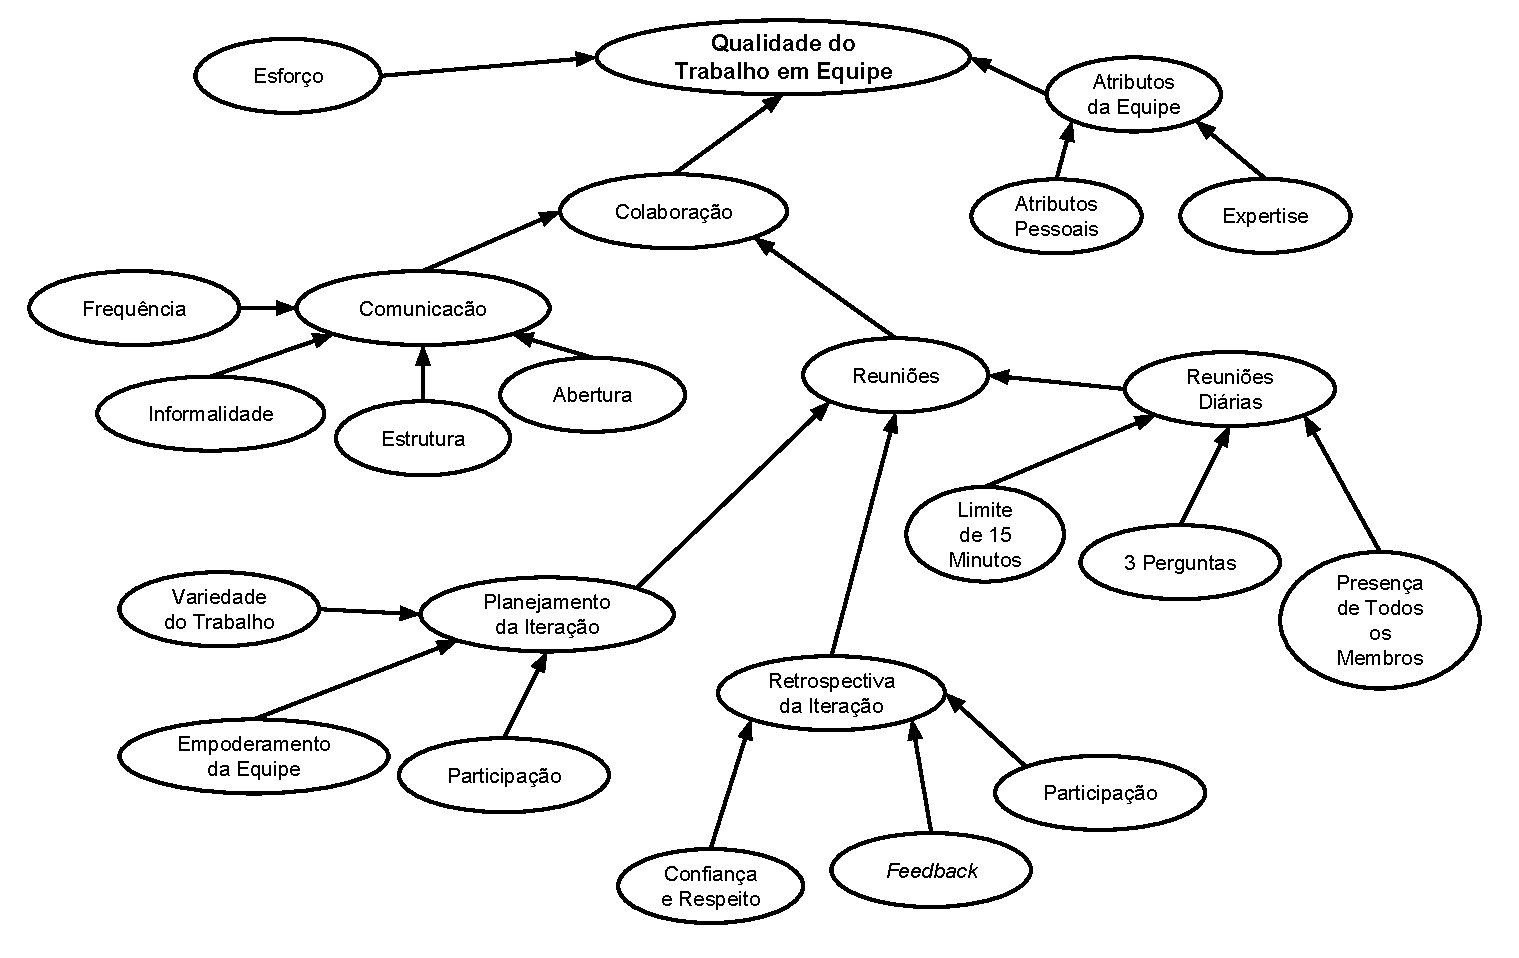
\includegraphics[scale=0.6]{figs/modeloSBES.pdf}}
	\end{center}
	\caption{Modelo Proposto por Freire et al.}
	\label{modelo:gad:freire}
\end{figure}

No modelo apresentado em \cite{freire}, a qualidade do TE depende diretamente de três principais nós: \textit{Colaboração}, \textit{Esforço} da equipe de desenvolvimento e \textit{Atributos da Equipe}. Entretanto, como foi decidido considerar o TE no contexto das relações entre os membros da equipe para alcançar os objetivos propostos, o nó \textit{Esforço} não se enquadra no contexto deste trabalho. Como é esperado que as equipes ágeis sejam auto-organizáveis \cite{manifesto}, o nó \textit{Esforço} foi substituído por \textit{Auto-Gerenciamento}. Dessa forma, o fator principal, \textit{Trabalho em Equipe}, passa a depender diretamente dos nós: \textit{Colaboração}, \textit{Auto-Gerenciamento} e \textit{Atributos da Equipe} (Figura \ref{modelo:gad:altonivel}).

\begin{figure}[ht!]
\begin{center}
		\fbox{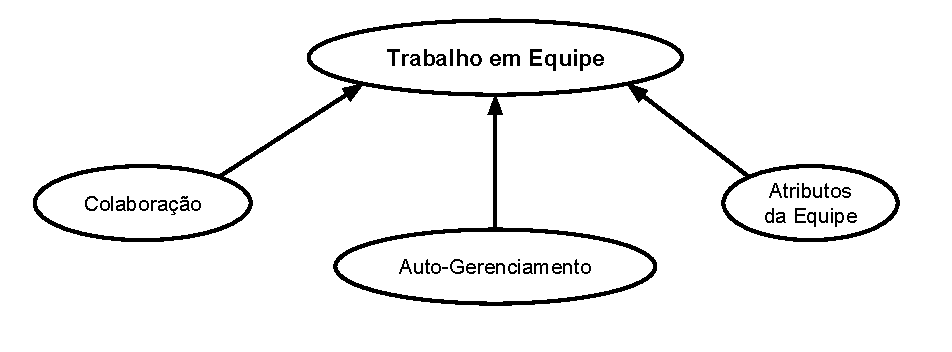
\includegraphics[scale=0.9]{figs/modeloAltoNivel.pdf}}
	\end{center}
	\caption{Representação do modelo proposto em alto nível.}
	\label{modelo:gad:altonivel}
\end{figure}

No modelo tomado como base, o nó \textit{Colaboração} depende diretamente dos nós \textit{Comunicação} e \textit{Reuniões}. \textit{Comunicação}, por sua vez, depende diretamente dos seguintes nós: \textit{Frequência}, \textit{Informalidade}, \textit{Estrutura} - possibilidade dos membros da equipe se comunicarem diretamente uns com os outros - e \textit{Abertura}, que está relacionada com o ato de não haver contenção de informação entre os membros da equipe. Como forma de minimizar a complexidade dos cálculos efetuados \cite{} e o viés que pode ser introduzido em virtude da subjetidade que esse nós representam, optou-se por substituir esses quatro nós por \textit{Distribuição da Equipe} e \textit{Cara-a-Cara}. Esse nós estão relacionados, respectivamente, com o fato dos membros da equipe compartilharem a mesma localidade e conversarem cara-a-cara diariamente. Dessa forma, a \textit{Distribuição da Equipe} substitui a \textit{Frequência}, uma vez que o fato de os membros da equipe compartilharem o mesmo local facilita a comunicação \cite{lalsing} e, assim, contribui para que a comunicação ocorra em maior frequência. Já o nó \textit{Cara-a-Cara} substitui a \textit{Informalidade}, \textit{Estrutura} e \textit{Abertura}, tendo em vista que essa prática contribui para que essas características se façam na presentes na \textit{Comunicação}.

O nó \textit{Reuniões}, que no modelo base depende diretamente dos nós \textit{Planejamento da Iteração}, \textit{Retrospectiva da Iteração} e \textit{Reuniões Diárias} foi substituído apenas pelo nó \textit{Reuniões Diárias}. Essa decisão foi tomada porque o que ocorre na \textit{Retrospectiva da Iteração} não influenciará mais o TE na iteração que se passou. O \textit{Planejamento da Iteração}, por sua vez, está relacionado com a utilização de técnicas de Engenharia de \textit{Software} que facilitam na prevenção contra riscos e estimativa de tempo para cumprimento de atividades. Além disso, não é objetivo do \textit{Planejamento da Iteração} melhorar a \textit{Comunicação} e a \textit{Colaboração} das equipes.

Conforme descrito em \cite{freire}, o nó \textit{Reuniões Diárias} depende diretamente dos seguintes nós: \textit{Limite de 15 Minutos}, \textit{3 Perguntas} (i.e., "O que eu fiz hoje?", "O que farei amanhã?" e "Quais obstáculos estão impedindo o meu progresso?") e \textit{Presença de Todos os Membros}. Entretanto, de acordo com Moe et al. \cite{moe2}, é necessário aplicar o \textit{Monitoramento} para que os membros da equipe observem as atividades e a eficiência dos outros integrantes, além de reconhecerem quando um membro da equipe atua corretamente, provendo \textit{feedback} e apoio. Logo, como o objetivo das perguntas é permitir aos participantes identificar potenciais barreiras e manter a coordenação da equipe, e isso está relacionando com o \textit{Monitoramento}, decidiu-se renomear o nó \textit{3 Perguntas} para \textit{Monitoramento}. Além disso, as três perguntas as quais o nó está relacionado são referentes ao contexto de \textit{Scrum}, e o modelo proposto neste trabalho é para avaliação do TE de equipes ágeis em geral. Também foi decidido remover o nó \textit{Limite de 15 minutos} porque ele não é considerado um indicador de qualidade dessas reuniões.

Em \cite{moe}, são descritos cinco fatores que precisam ser levados em conta para melhorar o TE de equipes ágeis. São eles: \textit{Liderança Compartilhada}, \textit{Orientação da Equipe}, \textit{Redundância}, \textit{Aprendizagem da Equipe} e \textit{Autonomia da Equipe}. A seguir, há a definição de cada um desses fatores com base nesse trabalho anteriormente citado:

\begin{itemize}
  \item \textit{Liderança Compartilhada}: Todos os membros da equipe compartilham a autoridade das decisões em vez centralizá-la. Dessa forma, evita que apenas uma pessoa tome as decisões, ou todos os membros da equipe tomem decisões levando em consideração apenas o seu trabalho individual, independente dos outros membros da equipe. Geralmente, o indivíduo que possui o conhecimento necessário durante uma determinada fase do projeto assume a liderança, compartilhando os seus conhecimentos, e permitindo que todos participem do processo de tomada de decisões;
  \item \textit{Orientação da Equipe}: Priorização dos objetivos da equipe em vez dos objetivos indivíduais, respeitando o compartamento de cada um dos membros da equipe;
  \item \textit{Redundância}: Os membros da equipe podem substituir uns aos outros sem treinamento extenso;
  \item \textit{Aprendizagem da Equipe}: Melhoria contínua dos métodos de trabalho com base nos \textit{feedbacks} fornecidos à equipe;
  \item \textit{Autonomia da Equipe}: As decisões tomadas pela equipe são respeitadas pelos gerentes que estão fora dela.
\end{itemize}

Ainda sobre as \textit{Reuniões Diárias}, durante elas, os membros da equipe tem a possibilidade de regular seus limites e condições, escolhendo em quais atividades desejam trabalhar, além de negociar e discutir sobre prevenção contra riscos e medidas corretivas. Como isso está relacionado à \textit{Autonomia da Equipe}, também foi decidido adicioná-lo como nó que influencia as \textit{Reuniões Diárias}. Dessa forma, tem-se que as \textit{Reuniões Diárias} tornam-se diretamente dependentes de \textit{Monitoramento}, \textit{Presença de Todos os Membros} e \textit{Autonomia da Equipe}.

Além disso, conforme supracitado, pode-se concluir que a \textit{Orientação da Equipe} contribui diretamente para a \textit{Colaboração} da equipe, pois há uma preocupação em priorizar os objetivos da equipe em vez dos objetivos individuais. Dessa forma, é necessário que os membros da equipes trabalhem de forma coesa, colaborando para que os objetivos da equipe sejam sempre alcançados. Por isso, decidiu-se adicionar o nó \textit{Orientação da Equipe} como influenciate do nó \textit{Colaboração}. Com isso, conforme representado na Figura \ref{modelo:gad:colaboracao}, o nó \textit{Colaboração} passa a depender diretamente dos nós \textit{Comunicação}, \textit{Orientação da Equipe} e \textit{Reuniões Diárias}.

\begin{figure}[ht!]
\begin{center}
		\fbox{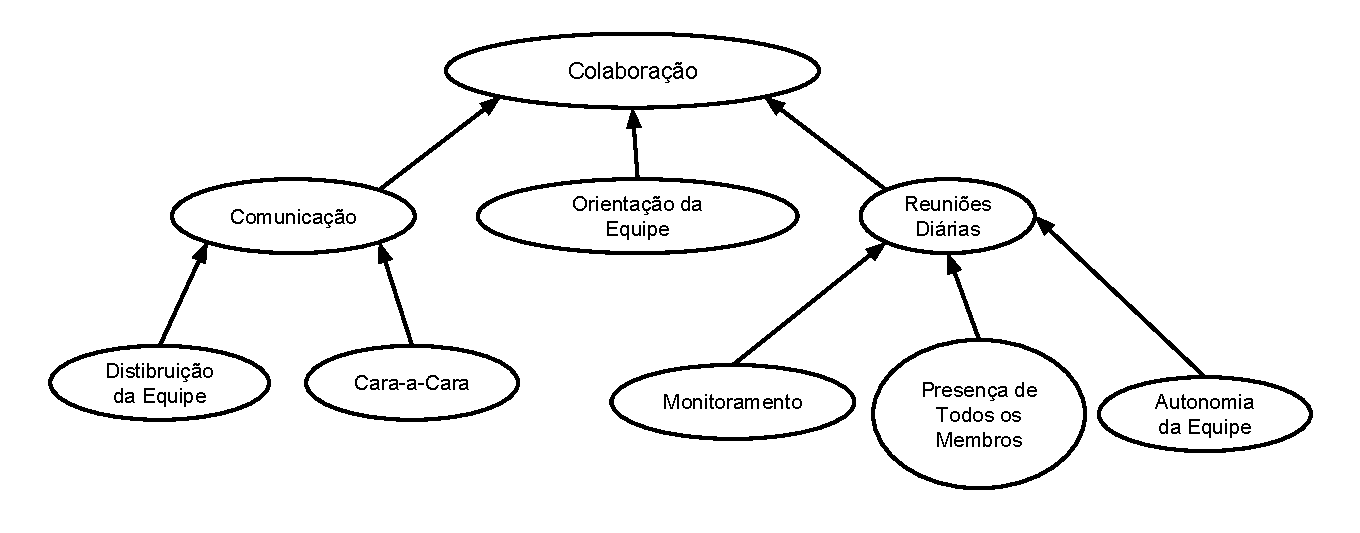
\includegraphics[scale=0.68]{figs/modeloColaboracao.pdf}}
	\end{center}
	\caption{Colaboração e os fatores que a influenciam.}
	\label{modelo:gad:colaboracao}
\end{figure}

\textit{Auto-Gerenciamento} é um dos novos nós que foi adicionado ao modelo, e influencia diretamente o TE. Na literatura, é estabelecido que a autoridade da decisão e da liderança de equipes auto-organizáveis precisa ser compartilhada \cite{morgan} \cite{kirkman}. Além disso, ainda em \cite{morgan}, é dito que equipes auto-organizáveis requerem uma capacidade de aprendizagem das equipes para que elas possam adaptar-se às transformações que ocorrem no ambiente. Ainda de acordo com \cite{morgan}, toda equipe que possui a capacidade de se auto-gerenciar precisa de um certo grau de \textit{Redundância}. Logo, com base nessas afirmações, os nós \textit{Liderança Compartilhada}, \textit{Aprendizagem da Equipe} e \textit{Redundância} foram adicionados como pais do nó \textit{Auto-Gerenciamento}. Na Figura \ref{modelo:gad:autogerenciamento} está representado o nó \textit{Auto-Gerenciamento} em conjunto com seus nós pai.

\begin{figure}[ht!]
\begin{center}
		\fbox{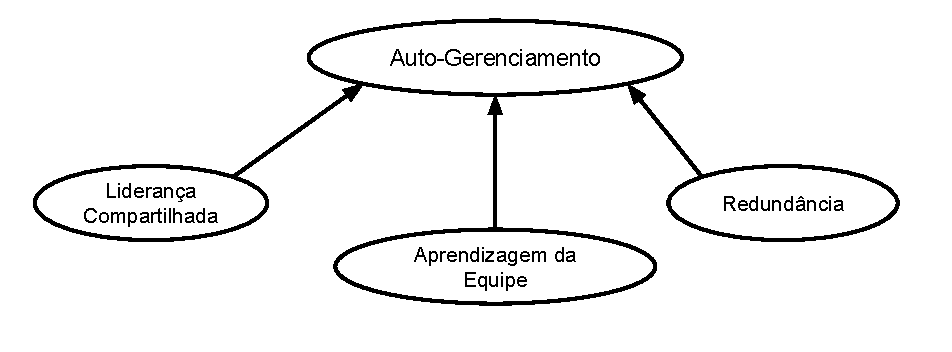
\includegraphics[scale=0.9]{figs/modeloAutoGerenciamento.pdf}}
	\end{center}
	\caption{Auto-Gerenciamento e os fatores que o influenciam.}
	\label{modelo:gad:autogerenciamento}
\end{figure}

O nó \textit{Atributos da Equipe} foi mantido como proposto no modelo em \cite{freire}. A Figura \ref{modelo:gad:atributos} contém a representação gráfica desse nó em particular.

\begin{figure}[ht!]
\begin{center}
		\fbox{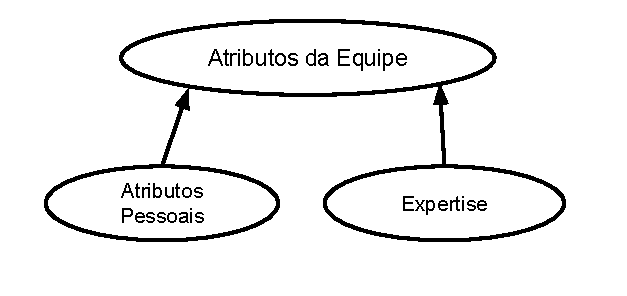
\includegraphics[scale=0.9]{figs/modeloAtributos.pdf}}
	\end{center}
	\caption{Atributos da Equipe e os fatores que o influenciam.}
	\label{modelo:gad:atributos}
\end{figure}

Finalmente, após definir os nós do GAD e os relacionamentos entre eles, na Figura \ref{modelo:gad:final} é possível verificar o GAD completo.

\begin{figure}[ht!]
\begin{center}
		\fbox{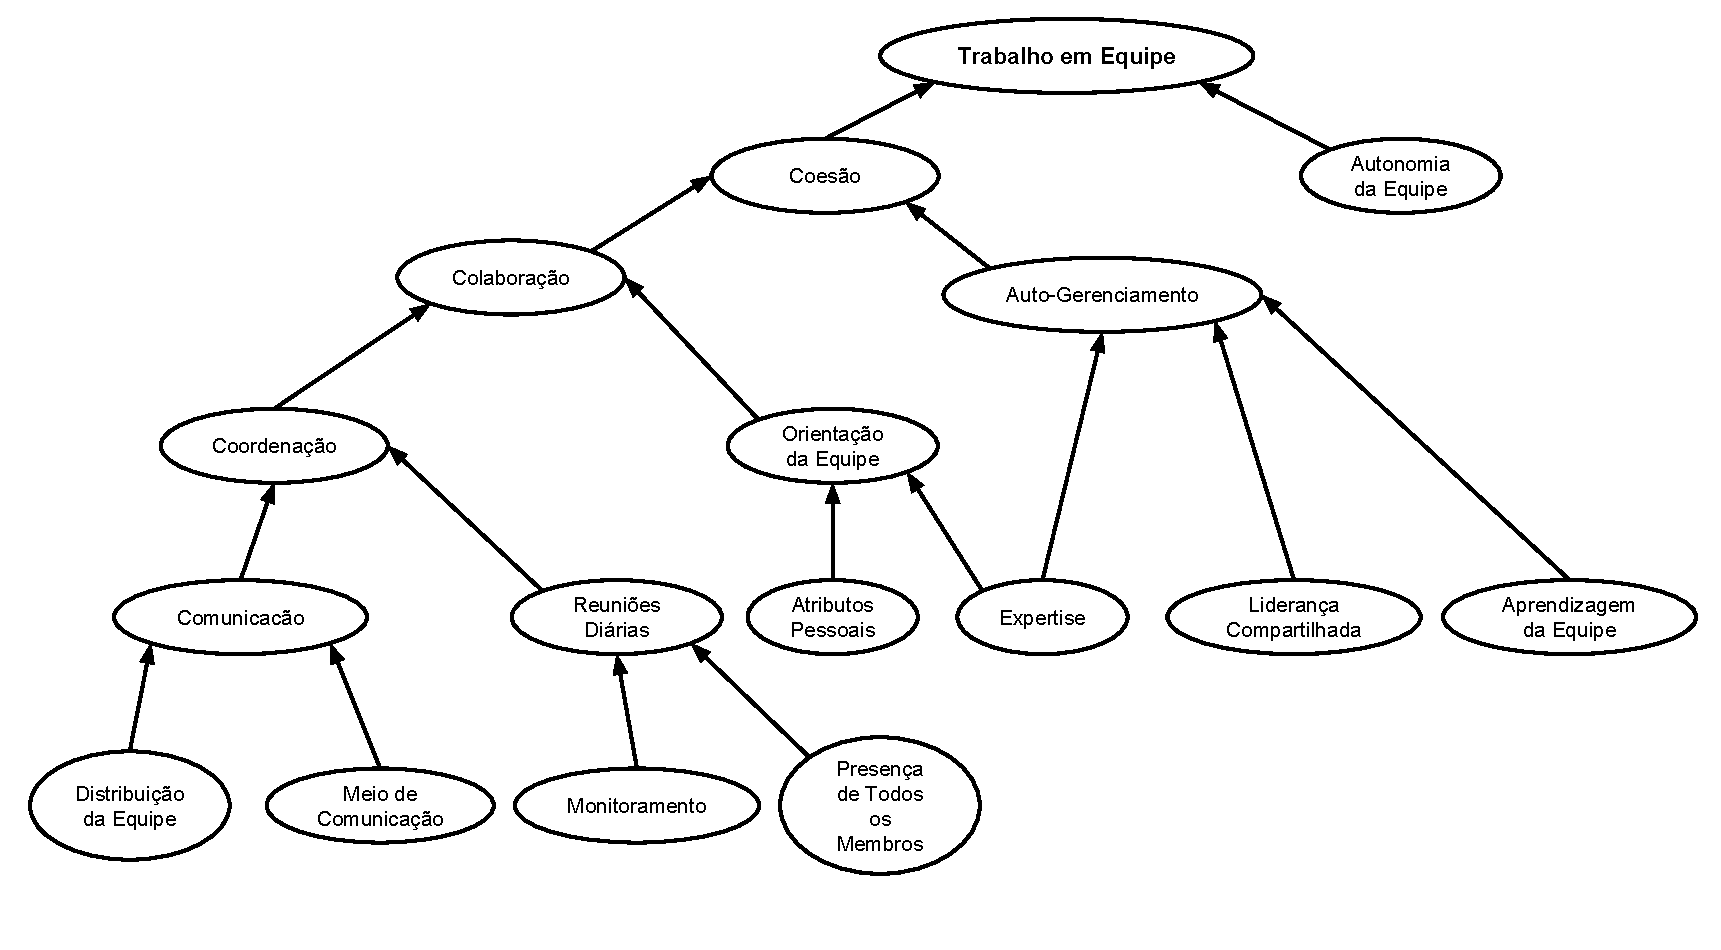
\includegraphics[scale=0.57]{figs/modeloFinal.pdf}}
	\end{center}
	\caption{Estrutura final do modelo proposto.}
	\label{modelo:gad:final}
\end{figure}

\section{Definição das Funções de Probabilidade}
\label{modelo:funcoes}

Apesar de \textit{Redes Bayesianas} serem úteis para resolverem problemas reais relacionados com risco e subjetividade, o seu uso ainda é restrito devido a dificuldade em definir as TPN. Há duas maneiras de se coletar dados para definir as TPN de uma \textit{Rede Bayesiana}: base de dados ou opinião de especialistas. Contudo, não é fácil encontrar uma base de dados adequada para um cenário específico de um problema prático. Por outro lado, a definição das TPN com a ajuda de especialistas requer bastante esforço (e.g., definir TPN para nós com um número muito alto de estados ou alta quantidade de pais, pois a quantidade de linhas de uma TPN aumenta exponencialmente em função da quantidade de pais do nó em questão). De acordo com Fenton et al. \cite{fenton}, isso pode acarretar em vários tipos de inconsistências no modelo.

Há vários métodos que têm como objetivo diminuir a complexidade e codificar a experiência de especialistas em grandes TPN. Noisy-OR \cite{huang} e Noisy-MAX \cite{diez} são dois desses métodos e possuem credibilidade. Contudo, Noisy-OR só pode ser aplicado a nós booleanos, e Noisy-MAX não é capaz de modelar o intervalo de relacionamentos que precisamos neste trabalho. Das \cite{das} propôs um algoritmo para popular as TPN que visa diminuir o tempo de duração para adquirir conhecimento de especialistas. Perkusich et al. \cite{perkusichNPT}, por sua vez, propõem um algoritmo cujo objetivo é ordenar os nós pai dadas as suas magnitudes relativas para o nó filho. Em seguida, com os nós pai ordenados por ordem de relevância, deve-se gerar as funções ponderadas com base na relevância dos nós pais e, finalmente, aplicá-las como funções de probabilidade dos nós.

Por outro lado, Fenton et al. \cite{fenton} propõem uma abordagem para \textit{Redes Bayesianas} que utiliza \textit{Nós Ranqueados}. Essa abordagem é baseada numa distribuição normal duplamente truncada (TNormal) que usa como média um tipo de função ponderada em função dos valores dos nós pai. Essa distribuição é baseada em quatro parâmetros: $u$, média (i.e., tendência central); $\sigma^{2}$, variância (i.e., confiança dos resultados); $a$, limite inferior (i.e., 0); e $b$, limite superior (i.e., 1). Essa distribuição permite que quem a utilize modele uma varidade de formas (i.e., relacionamentos). Por exemplo: uma distribuição uniforme ($\sigma^{2} = \infty$) e distribuições muito enviesadas ($\sigma^{2} = 0$). Na Figura \ref{modelo:funcoes:tnormal} há alguns exemplos de funções TNormal.


\begin{figure}[ht!]
\begin{center}
		\fbox{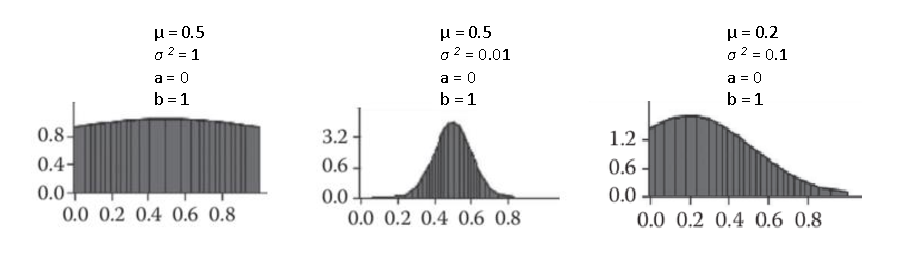
\includegraphics[scale=1]{figs/tnormalExemplos.pdf}}
	\end{center}
	\caption{Exemplos de Funções TNormal.}
	\label{modelo:funcoes:tnormal}
\end{figure}

Nessa abordagem, $u$ é definido por uma função ponderada baseada nos nós pai. Existem quatro tipos de funções ponderadas: média ponderada (WMEAN), mínimo ponderada (WMIN), máximo ponderada (WMAX) e uma última função que mescla a WMIN e a WMAX (MIXMINMAX). De acordo com os autores, essas funções são suficientes para representar os tipos de relações necessárias para definir as TPN. A Figura \ref{modelo:funcoes:ponderadas} contém exemplos de TPN calculadas com essas funções. Entretanto, apesar de WMEAN e MIXMINMAX apresentarem os mesmos valores, há uma diferença entre elas. A função WMEAN calcula a média ponderada dos nós pai, baseado nos pesos de cada nó pai, e a função MIXMINMAX mescla as funções WMIN e WMAX, também baseado nos pesos dos nós pai.

\begin{figure}[ht!]
\begin{center}
		\fbox{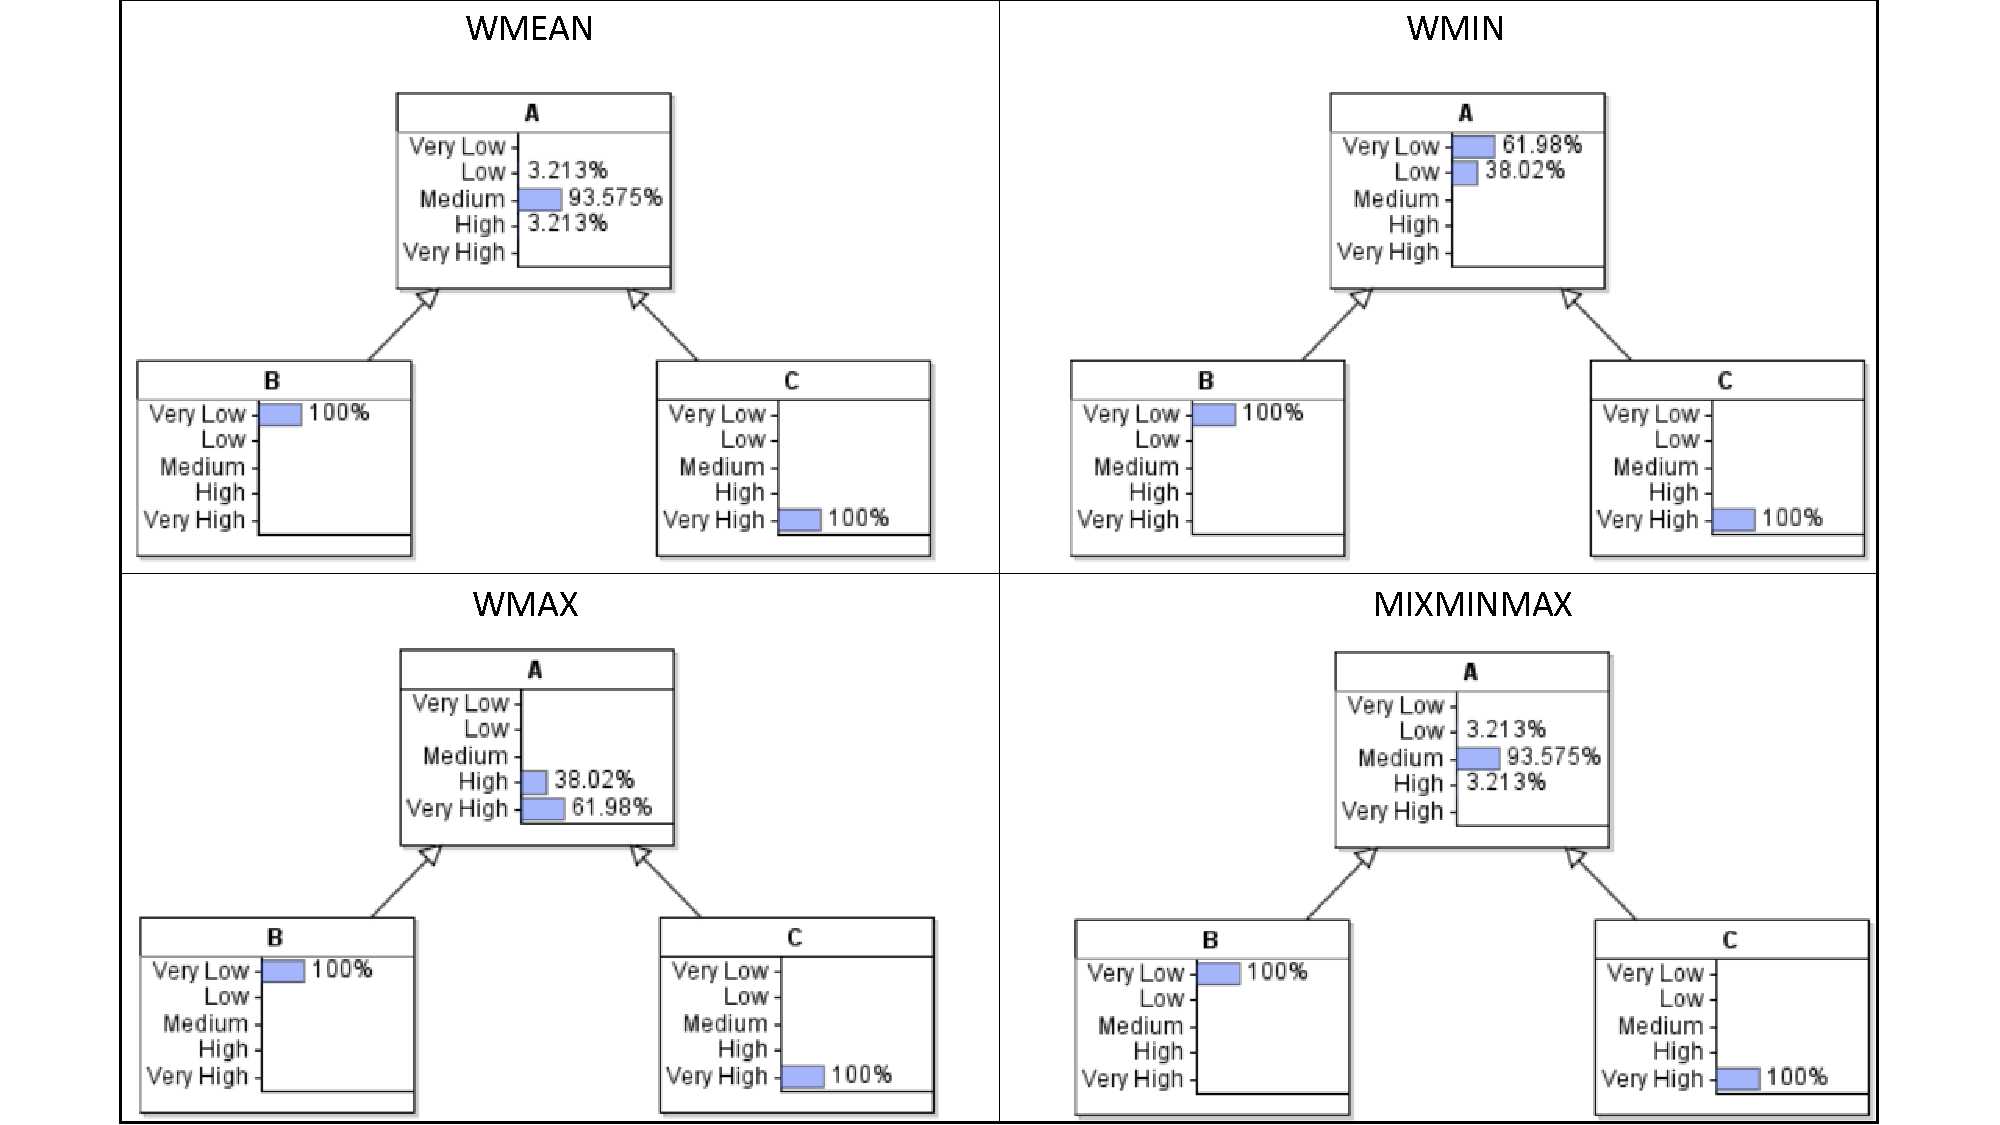
\includegraphics[scale=0.47]{figs/funcoesExemplos.pdf}}
	\end{center}
	\caption{Exemplos das Funções Ponderadas.}
	\label{modelo:funcoes:ponderadas}
\end{figure}

Para definir qual função deve ser utilizada, o indivíduo que está construindo o modelo deve definir perguntas para coletar respostas e definir as TPN. Tomando como base a \textit{Rede Bayesiana} representada na Figura \ref{modelo:funcoes:bn1}, um exemplo de pergunta seria: "Se o nó X1 for Muito Alto e o nó X2 for Muito Baixo, qual o valor esperado para o nó Y?". Baseado nas respostas, o indivíduo que está construindo a \textit{Rede Bayesiana} deve definir qual a função e quais os pesos adequados para definir as TPN. A variância deve ser definida empiricamente e deve refletir a confiança dos especialistas nos resultados.

\begin{figure}[ht!]
\begin{center}
		\fbox{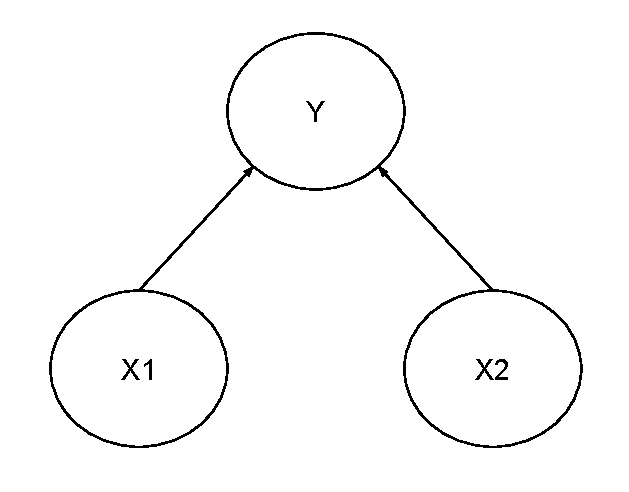
\includegraphics[scale=0.8]{figs/BN-2nos.pdf}}
	\end{center}
	\caption{Exemplo de nó filho com dois pais.}
	\label{modelo:funcoes:bn1}
\end{figure}

Entretanto, a base da abordagem proposta em \cite{fenton} consiste em mapear os estados dos nós em uma escala numérica. Logo, quanto menos precisa a tendência central do nó filho, mais vaga será a distribuição da função atribuida. Como forma de mitigar esses problemas, em \cite{laitila} é proposta uma abordagem similar. Contudo, nessa abordagem, em vez do especialista avaliar a função de probabilidade de um determinado nó filho atribuindo a qual dos estados desse nó a tendência central corresponde, são atríbuidas probabilidades para cada um dos estados do nó filho - a soma dessas probabilidades deve ser igual a 1. De acordo com os autores, essa abordagem provê uma transparência maior na elicitação dos pesos dos nós pai na função ponderada. Portanto, decidiu-se utilizar essa abordagem para definir as funções de probabilidade do modelo proposto.

Um especialista em \textit{Redes Bayesianas} e Métodos Ágeis foi o responsável por realizar essa atividade. Para cada nó filho, o especialista deve definir quais as probabilidades desse nó estar em cada estado, com base nos estados dos nós pai. Portanto, para um nó com dois pais, e tomando como exemplo a \textit{Rede Bayesiana} apresentada na Figura \ref{modelo:funcoes:bn1}, o especialista precisou preencher as células em branco da Tabela \ref{modelo:funcoes:tabela2nos} com os valores esperados, de forma que, para cada combinação possível

\begin{align}
  \sum_{i=1}^{n}Pi = 1,\\ \intertext{onde $Pi$ é a probabilidade de cada estado e $n$ é a quantidade de estados possíveis do nó filho}
\end{align}

\begin{table}[ht!]
\centering
\caption{Tabela para definição das Funções de Probabilidade de nós com dois pais.}
\label{modelo:funcoes:tabela2nos}
\begin{tabular}{|c|c|c|c|c|c|c|}
\hline
\multicolumn{2}{|l|}{}                      & \multicolumn{5}{c|}{\textbf{Valores Esperados para Y}}                                       \\ \hline
\textbf{X1}          & \textbf{X2}          & \textbf{Muito Baixa} & \textbf{Baixa} & \textbf{Média} & \textbf{Alta} & \textbf{Muito Alta} \\ \hline
\textbf{Muito Alta}  & \textbf{Muito Baixa} & $P_{1}$              & $P_{2}$        & $P_{3}$        & $P_{4}$       & $P_{5}$              \\ \hline
\textbf{Muito Baixa} & \textbf{Muito Alta}  & $P_{1}$              & $P_{2}$        & $P_{3}$        & $P_{4}$       & $P_{5}$             \\ \hline
\textbf{Muito Alta}  & \textbf{Média}       & $P_{1}$              & $P_{2}$        & $P_{3}$        & $P_{4}$       & $P_{5}$             \\ \hline
\textbf{Média}       & \textbf{Muito Alta}  & $P_{1}$              & $P_{2}$        & $P_{3}$        & $P_{4}$       & $P_{5}$             \\ \hline
\end{tabular}
\end{table}

De maneira análoga, para cada nó filho com três pais (e.g., Figura \ref{modelo:funcoes:bn2}), porém com uma maior quantidade de combinações possíveis, o especialista precisou preencher as células em branco de uma similar à Tabela \ref{modelo:funcoes:tabela3nos}.

\begin{figure}[ht!]
\begin{center}
		\fbox{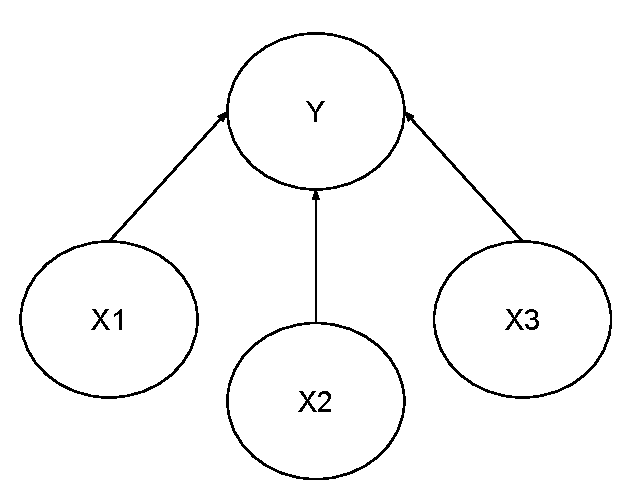
\includegraphics[scale=0.8]{figs/BN-3nos.pdf}}
	\end{center}
	\caption{Exemplo de nó filho com três pais.}
	\label{modelo:funcoes:bn2}
\end{figure}

\begin{table}[ht!]
\centering
\caption{Tabela para definição das Funções de Probabilidade de nós com três pais.}
\label{modelo:funcoes:tabela3nos}
\resizebox{\textwidth}{!}{\begin{tabular}{|c|c|c|c|c|c|c|c|}
\hline
\multicolumn{3}{|c|}{}                                             & \multicolumn{5}{c|}{\textbf{Valores Esperados para Y}}                                       \\ \hline
\textbf{X1}          & \textbf{X2}          & \textbf{X3}          & \textbf{Muito Baixa} & \textbf{Baixa} & \textbf{Média} & \textbf{Alta} & \textbf{Muito Alta} \\ \hline
\textbf{Muito Alta}  & \textbf{Muito Alta}  & \textbf{Muito Baixa} & $P_{1}$              & $P_{2}$        & $P_{3}$        & $P_{4}$       & $P_{5}$              \\ \hline
\textbf{Muito Alta}  & \textbf{Muito Baixa} & \textbf{Muito Alta}  & $P_{1}$              & $P_{2}$        & $P_{3}$        & $P_{4}$       & $P_{5}$              \\ \hline
\textbf{Muito Baixa} & \textbf{Muito Alta}  & \textbf{Muito Alta}  & $P_{1}$              & $P_{2}$        & $P_{3}$        & $P_{4}$       & $P_{5}$              \\ \hline
\textbf{Muito Baixa} & \textbf{Muito Baixa} & \textbf{Muito Alta}  & $P_{1}$              & $P_{2}$        & $P_{3}$        & $P_{4}$       & $P_{5}$              \\ \hline
\textbf{Muito Baixa} & \textbf{Muito Alta}  & \textbf{Muito Baixa} & $P_{1}$              & $P_{2}$        & $P_{3}$        & $P_{4}$       & $P_{5}$              \\ \hline
\textbf{Muito Alta}  & \textbf{Muito Baixa} & \textbf{Muito Baixa} & $P_{1}$              & $P_{2}$        & $P_{3}$        & $P_{4}$       & $P_{5}$              \\ \hline
\end{tabular}}
\end{table}

Assim, de acordo com a quantidade de nós pai de um determinado nó, foram definidas tabelas para cada um dos nós presentes no modelo proposto, exceto os nós de entrada. Uma vez que essas tabelas foram definidas, o especialista, com a ajuda de uma ferramenta, calculou os resultados reais para cada estado. Esses cálculos foram feitos diversas vezes, pois há a necessidade de definir qual função ponderada representa a tabela de probabilidade do nó em questão, além dos pesos de cada um dos nós pai praquela função. Esses cálculos são realizados diversas vezes até que a função e os pesos adequados, que mais se aproximem dos valores esperados, sejam encontrados. Além disso, o processo de definição das funções de probabilidade por parte do especialista é muito importante, pois caso haja inconsistências na definição do GAD, é necessário reorgarnizar a estrutura do grafo para garantir a consistência entre os conceitos e relacionamentos que estão sendo representados. Finalmente, ao final desse processo, o modelo está pronto para ser utilizado. A Tabela \ref{modelo:funcoes:tabelapesos} contém as funções e os pesos dos nós pai de todos os nós do modelo, exceto os nós de entrada.

\begin{table}[ht!]
\centering
\caption{Definição das Funções de Probabilidade.}
\label{modelo:funcoes:tabelapesos}
\resizebox{\textwidth}{!}{\begin{tabular}{|c|c|c|c|c|c|c|c|c|}
\hline
\multicolumn{3}{|c|}{\textbf{}}                                                                                                      & \multicolumn{3}{c|}{\textbf{Pais}}                                                                                                                                                                            & \multicolumn{3}{c|}{\textbf{Pesos}}                                      \\ \hline
\textbf{Nó}                                                              & \textbf{Função} & \multicolumn{1}{l|}{\textbf{Variância}} & \textbf{Pai 2}                                                    & \textbf{Pai 2}                                                         & \textbf{Pai 3}                                                   & \textbf{Peso do Pai 1} & \textbf{Peso do Pai 2} & \textbf{Peso do Pai 3} \\ \hline
\textbf{Trabalho em Equipe}                                              & wmin            & 0,0005                                  & Colaboração                                                       & Auto-Gerenciamento                                                     & \begin{tabular}[c]{@{}c@{}}Autonomia \\ da Equipe\end{tabular}   & 10                     & 10                     & 10                     \\ \hline
\textbf{Colaboração}                                                     & wmin            & 0,0005                                  & Comunicação                                                       & Reuniões Diárias                                                       & \begin{tabular}[c]{@{}c@{}}Orientação \\ da Equipe\end{tabular}  & 10                     & 10                     & 10                     \\ \hline
\textbf{Auto-Gerenciamento}                                              & wmin            & 0,0005                                  & Expertise                                                         & \begin{tabular}[c]{@{}c@{}}Liderança \\ Compartilhada\end{tabular}     & \begin{tabular}[c]{@{}c@{}}Aprendizagem\\ da Equipe\end{tabular} & 3                      & 2                      & 1                      \\ \hline
\textbf{Comunicação}                                                     & wmin            & 0,0005                                  & \begin{tabular}[c]{@{}c@{}}Distribuição \\ da Equipe\end{tabular} & \begin{tabular}[c]{@{}c@{}}Meio \\ de Comunicação\end{tabular}         & X                                                                & 3                      & 5                      & X                      \\ \hline
\textbf{Reuniões Diárias}                                                & wmin            & 0,0005                                  & Monitoramento                                                     & \begin{tabular}[c]{@{}c@{}}Presença de Todos\\ os Membros\end{tabular} & X                                                                & 7                      & 7                      & X                      \\ \hline
\textbf{\begin{tabular}[c]{@{}c@{}}Orientação \\ da Equipe\end{tabular}} & wmin            & 0,0005                                  & \begin{tabular}[c]{@{}c@{}}Atributos \\ Pessoais\end{tabular}     & Expertise                                                              & X                                                                & 5                      & 5                      & X                      \\ \hline
\end{tabular}}
\end{table}
